\documentclass[border=1cm]{standalone}
\usepackage{tikz}
\usepackage{tkz-euclide}
\usetikzlibrary{patterns}
\begin{document}
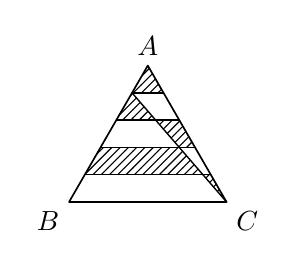
\begin{tikzpicture}[scale=.5]
    \tkzDefPoint(0,0){B} 
    \tkzDefPoint(4,0){C}
    \tkzDefPoint(2,2*sqrt(3)){A}
    \tkzDrawPolygon[line width = .6pt](A,B,C)
    \tkzLabelPoints[above](A)
    \tkzLabelPoints[below left](B)
    \tkzLabelPoints[below right](C)
    \tkzDefPointWith[linear,K=.2](A,B)
    \tkzGetPoint{M1}
    \tkzDefPointWith[linear,K=.4](A,B)
    \tkzGetPoint{M2}
    \tkzDefPointWith[linear,K=.6](A,B)
    \tkzGetPoint{M3}
    \tkzDefPointWith[linear,K=.8](A,B)
    \tkzGetPoint{M4}
    \tkzDefPointWith[linear,K=.2](A,C)
    \tkzGetPoint{N1}
    \tkzDefPointWith[linear,K=.4](A,C)
    \tkzGetPoint{N2}
    \tkzDefPointWith[linear,K=.6](A,C)
    \tkzGetPoint{N3}
    \tkzDefPointWith[linear,K=.8](A,C)
    \tkzGetPoint{N4}
    \tkzDrawSegments[line width = .5pt](M1,N1 M2,N2 M3,N3 M4,N4 M1,C)
    \tkzInterLL(M1,C)(M2,N2)
    \tkzGetPoint{I1}
    \tkzInterLL(M1,C)(M3,N3)
    \tkzGetPoint{I2}
    \tkzInterLL(M1,C)(M4,N4)
    \tkzGetPoint{I3}
    \tkzFillPolygon[pattern={north east lines}](A,M1,N1)
    \tkzFillPolygon[pattern={north east lines}](A,M1,M2)
    \tkzFillPolygon[pattern={north east lines}](M1,M2,I1)
    \tkzFillPolygon[pattern={north east lines}](I1,N2,N3,I2)
    \tkzFillPolygon[pattern={north east lines}](M3,I2,I3,M4)
    \tkzFillPolygon[pattern={north east lines}](I3,N4,C)
    \end{tikzpicture}
\end{document}